% Options for packages loaded elsewhere
\PassOptionsToPackage{unicode}{hyperref}
\PassOptionsToPackage{hyphens}{url}
\PassOptionsToPackage{dvipsnames,svgnames,x11names}{xcolor}
%
\documentclass[
]{article}

\usepackage{amsmath,amssymb}
\usepackage{iftex}
\ifPDFTeX
  \usepackage[T1]{fontenc}
  \usepackage[utf8]{inputenc}
  \usepackage{textcomp} % provide euro and other symbols
\else % if luatex or xetex
  \usepackage{unicode-math}
  \defaultfontfeatures{Scale=MatchLowercase}
  \defaultfontfeatures[\rmfamily]{Ligatures=TeX,Scale=1}
\fi
\usepackage[]{times}
\ifPDFTeX\else  
    % xetex/luatex font selection
\fi
% Use upquote if available, for straight quotes in verbatim environments
\IfFileExists{upquote.sty}{\usepackage{upquote}}{}
\IfFileExists{microtype.sty}{% use microtype if available
  \usepackage[]{microtype}
  \UseMicrotypeSet[protrusion]{basicmath} % disable protrusion for tt fonts
}{}
\makeatletter
\@ifundefined{KOMAClassName}{% if non-KOMA class
  \IfFileExists{parskip.sty}{%
    \usepackage{parskip}
  }{% else
    \setlength{\parindent}{0pt}
    \setlength{\parskip}{6pt plus 2pt minus 1pt}}
}{% if KOMA class
  \KOMAoptions{parskip=half}}
\makeatother
\usepackage{xcolor}
\setlength{\emergencystretch}{3em} % prevent overfull lines
\setcounter{secnumdepth}{2}
% Make \paragraph and \subparagraph free-standing
\makeatletter
\ifx\paragraph\undefined\else
  \let\oldparagraph\paragraph
  \renewcommand{\paragraph}{
    \@ifstar
      \xxxParagraphStar
      \xxxParagraphNoStar
  }
  \newcommand{\xxxParagraphStar}[1]{\oldparagraph*{#1}\mbox{}}
  \newcommand{\xxxParagraphNoStar}[1]{\oldparagraph{#1}\mbox{}}
\fi
\ifx\subparagraph\undefined\else
  \let\oldsubparagraph\subparagraph
  \renewcommand{\subparagraph}{
    \@ifstar
      \xxxSubParagraphStar
      \xxxSubParagraphNoStar
  }
  \newcommand{\xxxSubParagraphStar}[1]{\oldsubparagraph*{#1}\mbox{}}
  \newcommand{\xxxSubParagraphNoStar}[1]{\oldsubparagraph{#1}\mbox{}}
\fi
\makeatother


\providecommand{\tightlist}{%
  \setlength{\itemsep}{0pt}\setlength{\parskip}{0pt}}\usepackage{longtable,booktabs,array}
\usepackage{calc} % for calculating minipage widths
% Correct order of tables after \paragraph or \subparagraph
\usepackage{etoolbox}
\makeatletter
\patchcmd\longtable{\par}{\if@noskipsec\mbox{}\fi\par}{}{}
\makeatother
% Allow footnotes in longtable head/foot
\IfFileExists{footnotehyper.sty}{\usepackage{footnotehyper}}{\usepackage{footnote}}
\makesavenoteenv{longtable}
\usepackage{graphicx}
\makeatletter
\def\maxwidth{\ifdim\Gin@nat@width>\linewidth\linewidth\else\Gin@nat@width\fi}
\def\maxheight{\ifdim\Gin@nat@height>\textheight\textheight\else\Gin@nat@height\fi}
\makeatother
% Scale images if necessary, so that they will not overflow the page
% margins by default, and it is still possible to overwrite the defaults
% using explicit options in \includegraphics[width, height, ...]{}
\setkeys{Gin}{width=\maxwidth,height=\maxheight,keepaspectratio}
% Set default figure placement to htbp
\makeatletter
\def\fps@figure{htbp}
\makeatother
% definitions for citeproc citations
\NewDocumentCommand\citeproctext{}{}
\NewDocumentCommand\citeproc{mm}{%
  \begingroup\def\citeproctext{#2}\cite{#1}\endgroup}
\makeatletter
 % allow citations to break across lines
 \let\@cite@ofmt\@firstofone
 % avoid brackets around text for \cite:
 \def\@biblabel#1{}
 \def\@cite#1#2{{#1\if@tempswa , #2\fi}}
\makeatother
\newlength{\cslhangindent}
\setlength{\cslhangindent}{1.5em}
\newlength{\csllabelwidth}
\setlength{\csllabelwidth}{3em}
\newenvironment{CSLReferences}[2] % #1 hanging-indent, #2 entry-spacing
 {\begin{list}{}{%
  \setlength{\itemindent}{0pt}
  \setlength{\leftmargin}{0pt}
  \setlength{\parsep}{0pt}
  % turn on hanging indent if param 1 is 1
  \ifodd #1
   \setlength{\leftmargin}{\cslhangindent}
   \setlength{\itemindent}{-1\cslhangindent}
  \fi
  % set entry spacing
  \setlength{\itemsep}{#2\baselineskip}}}
 {\end{list}}
\usepackage{calc}
\newcommand{\CSLBlock}[1]{\hfill\break\parbox[t]{\linewidth}{\strut\ignorespaces#1\strut}}
\newcommand{\CSLLeftMargin}[1]{\parbox[t]{\csllabelwidth}{\strut#1\strut}}
\newcommand{\CSLRightInline}[1]{\parbox[t]{\linewidth - \csllabelwidth}{\strut#1\strut}}
\newcommand{\CSLIndent}[1]{\hspace{\cslhangindent}#1}

% Place figures and tables exactly where they were called
\usepackage{float}
\floatplacement{figure}{H}
\floatplacement{table}{H}

% Recommended by the modelsummary package
\usepackage{booktabs}
\usepackage{siunitx}
\newcolumntype{d}{S[input-symbols = ()]}

% Add affiliations (title.tex needs to be called under template-partials)
\usepackage[noblocks]{authblk}
\renewcommand*{\Authsep}{, }
\renewcommand*{\Authand}{, }
\renewcommand*{\Authands}{, }
\renewcommand\Affilfont{\small}

% Add line numbers
\usepackage{lineno}
\linenumbers
\usepackage{float}
\usepackage{tabularray}
\usepackage[normalem]{ulem}
\usepackage{graphicx}
\UseTblrLibrary{booktabs}
\UseTblrLibrary{siunitx}
\NewTableCommand{\tinytableDefineColor}[3]{\definecolor{#1}{#2}{#3}}
\newcommand{\tinytableTabularrayUnderline}[1]{\underline{#1}}
\newcommand{\tinytableTabularrayStrikeout}[1]{\sout{#1}}
\makeatletter
\@ifpackageloaded{caption}{}{\usepackage{caption}}
\AtBeginDocument{%
\ifdefined\contentsname
  \renewcommand*\contentsname{Table of contents}
\else
  \newcommand\contentsname{Table of contents}
\fi
\ifdefined\listfigurename
  \renewcommand*\listfigurename{List of Figures}
\else
  \newcommand\listfigurename{List of Figures}
\fi
\ifdefined\listtablename
  \renewcommand*\listtablename{List of Tables}
\else
  \newcommand\listtablename{List of Tables}
\fi
\ifdefined\figurename
  \renewcommand*\figurename{Figure}
\else
  \newcommand\figurename{Figure}
\fi
\ifdefined\tablename
  \renewcommand*\tablename{Table}
\else
  \newcommand\tablename{Table}
\fi
}
\@ifpackageloaded{float}{}{\usepackage{float}}
\floatstyle{ruled}
\@ifundefined{c@chapter}{\newfloat{codelisting}{h}{lop}}{\newfloat{codelisting}{h}{lop}[chapter]}
\floatname{codelisting}{Listing}
\newcommand*\listoflistings{\listof{codelisting}{List of Listings}}
\makeatother
\makeatletter
\makeatother
\makeatletter
\@ifpackageloaded{caption}{}{\usepackage{caption}}
\@ifpackageloaded{subcaption}{}{\usepackage{subcaption}}
\makeatother

\ifLuaTeX
  \usepackage{selnolig}  % disable illegal ligatures
\fi
\usepackage{bookmark}

\IfFileExists{xurl.sty}{\usepackage{xurl}}{} % add URL line breaks if available
\urlstyle{same} % disable monospaced font for URLs
\hypersetup{
  pdftitle={The Impact of Weather on Flight Delay},
  pdfauthor={Forgot MyName; No Name},
  pdfkeywords={Reproducible, R},
  colorlinks=true,
  linkcolor={blue},
  filecolor={Maroon},
  citecolor={red},
  urlcolor={Blue},
  pdfcreator={LaTeX via pandoc}}


\title{The Impact of Weather on Flight Delay}


  \author{Forgot MyName}
            \affil{%
                  Random University
              }
        \author{No Name}
            \affil{%
                  Highest-ranked University
              }
      
\date{2024-10-16}
\begin{document}
\maketitle
\begin{abstract}
Abstract: this research is so awesome that you cannot reject this paper.
\end{abstract}


\section{Introduction}\label{introduction}

Nothing is more frustrating than flight delays. The goal of this article
is to understand what weather variables affect flights delays so that we
can control weather when such time comes in the future\footnote{This is
  just for illustrating how to create a footnote}.

\section{Method}\label{method}

Regression analysis was used in this article. The econometric model
writes as follows (equation \ref{econometric-model})):

\begin{align}
y_{i,t} = \beta_0 + \beta_1 temp_{i,t} + \beta_2 precip_{i,t} + \beta_3 wind_speed_{i,t} + v_{i,t} \lable{econometric-model}
\end{align}

\subsection{Code availability}\label{code-availability}

All computations (including creating tables and plots) were conducted
using R software (\citeproc{ref-R}{R Core Team 2022}), The Bergé
(\citeproc{ref-fixest}{2018}) package was used to run regressions.

\section{Data}\label{data}

We use publicly available datasets from the R \texttt{nycflights13}
package (\citeproc{ref-nycflights13}{Wickham 2021}).
\textbf{?@tbl-sum-stat} presents the summary statistics.

\begin{table}
\caption{Summary Statistics}\tabularnewline

\centering
\begin{tblr}[         %% tabularray outer open
]                     %% tabularray outer close
{                     %% tabularray inner open
colspec={Q[]Q[]Q[]Q[]},
column{1}={halign=l,},
column{2}={halign=r,},
column{3}={halign=r,},
column{4}={halign=r,},
}                     %% tabularray inner close
\toprule
& Mean & SD & Max \\ \midrule %% TinyTableHeader
dep\_delay  & \num{12.64} & \num{40.21} & \num{1301.00} \\
temp         & \num{55.57} & \num{17.10} & \num{92.14}   \\
precip       & \num{0.00}  & \num{0.01}  & \num{0.15}    \\
wind\_speed & \num{10.45} & \num{4.19}  & \num{56.39}   \\
\bottomrule
\end{tblr}
\end{table}

Figure \textbf{?@fig-hist-delay} shows the histogram of departure delay
by carrier for each of the airports.

\begin{figure}[H]

{\centering 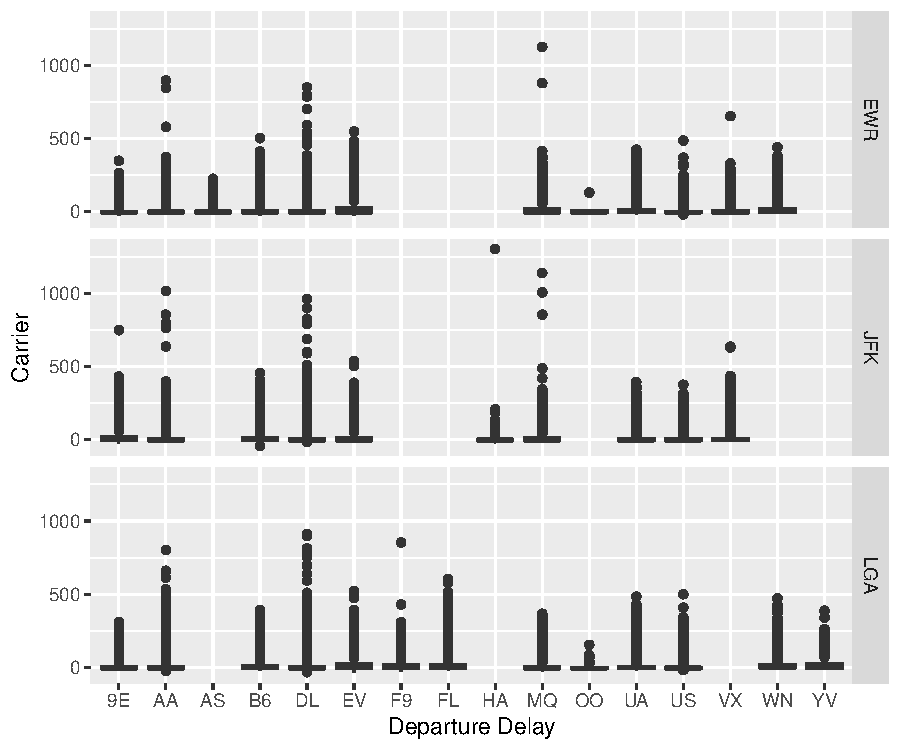
\includegraphics{../results/figures/delay_box.pdf}

}

\caption{Distribution of delay by carrier}

\end{figure}%

\section{Results and Discussions}\label{results-and-discussions}

\textbf{?@tbl-reg-results} presents the regression results.

\begin{table}
\caption{Regression Results}\tabularnewline

\centering
\begin{talltblr}[         %% tabularray outer open
entry=none,label=none,
note{}={+ p < 0.1, * p < 0.05, ** p < 0.01, *** p < 0.001},
]                     %% tabularray outer close
{                     %% tabularray inner open
colspec={Q[]Q[]Q[]Q[]},
column{1}={halign=l,},
column{2}={halign=c,},
column{3}={halign=c,},
column{4}={halign=c,},
hline{10}={1,2,3,4}{solid, 0.05em, black},
}                     %% tabularray inner close
\toprule
& (1) & (2) & (3) \\ \midrule %% TinyTableHeader
(Intercept)  & \num{0.068}      &                  &                  \\
& (\num{0.348})    &                  &                  \\
temp         & \num{0.145}***   & \num{0.251}+    & \num{0.251}**   \\
& (\num{0.004})    & (\num{0.125})   & (\num{0.023})   \\
precip       & \num{379.641}*** & \num{348.979}** & \num{348.979}** \\
& (\num{5.363})    & (\num{105.112}) & (\num{28.751})  \\
wind\_speed & \num{0.274}***   & \num{0.326}+    & \num{0.326}*    \\
& (\num{0.018})    & (\num{0.155})   & (\num{0.059})   \\
Num.Obs.     & \num{326164}     & \num{326164}    & \num{326164}    \\
R2           & \num{0.020}      & \num{0.034}     & \num{0.034}     \\
Std.Errors   & IID               & by: month        & by: origin       \\
\bottomrule
\end{talltblr}
\end{table}

\section{Conclusion}\label{conclusion}

Weather matters.

\section*{References}\label{references}
\addcontentsline{toc}{section}{References}

\phantomsection\label{refs}
\begin{CSLReferences}{1}{0}
\bibitem[\citeproctext]{ref-fixest}
Bergé, Laurent, {``Efficient estimation of maximum likelihood models
with multiple fixed-effects: The {R} package {FENmlm},''} \emph{CREA
Discussion Papers}, (2018).

\bibitem[\citeproctext]{ref-R}
R Core Team, {``\href{https://www.R-project.org/}{R: A language and
environment for statistical computing},''} (Vienna, Austria, R
Foundation for Statistical Computing, 2022).

\bibitem[\citeproctext]{ref-nycflights13}
Wickham, Hadley,
{``\href{https://CRAN.R-project.org/package=nycflights13}{nycflights13:
Flights that departed NYC in 2013},''} (2021).

\end{CSLReferences}




\end{document}
